\documentclass[10pt,a4paper]{article}
\usepackage[margin=0.5in]{geometry}
\usepackage[utf8]{inputenc}
\usepackage[english]{babel}
\usepackage{amsmath}
\usepackage{amsfonts}
\usepackage{amssymb}
\usepackage{cancel}
\usepackage{xcolor}
\usepackage{graphicx}
\usepackage{hyperref}


%\renewcommand\CancelColor{<color command>}
\newcommand\cc[2][black]{\renewcommand\CancelColor{\color{#1}}\cancel{#2}}
\newcommand{\ud}[1]{\underline{#1}}
\DeclareMathOperator{\tm}{\times}
\DeclareMathOperator{\cross}{\wedge}
\DeclareMathOperator{\AD}{\ud{AD}}
\DeclareMathOperator{\AC}{\ud{AC}}
\DeclareMathOperator{\CD}{\ud{CD}}
\DeclareMathOperator{\AO}{\ud{AO}}
\DeclareMathOperator{\OA}{\ud{OA}}
\DeclareMathOperator{\OD}{\ud{OD}}
\DeclareMathOperator{\ED}{\ud{ED}}
\DeclareMathOperator{\eA}{\ud{e}_A}
\DeclareMathOperator{\eB}{\ud{e}_B}
\DeclareMathOperator{\n}{\ud{n}}
\DeclareMathOperator{\z}{\ud{z}}
\DeclareMathOperator{\ODz}{\|\OD \cross  \z\|}
\DeclareMathOperator{\OAz2}{\|\OA \cross  \z\|^2}
\DeclareMathOperator{\eAz2}{\|\eA \cross  \z\|^2}
\DeclareMathOperator{\ODn}{\|\ud{OD}\|}
\DeclareMathOperator{\ra}{r_{a}}
\DeclareMathOperator{\ea}{\ud{e}_{a}}
\DeclareMathOperator{\rb}{r_{b}}


\title{Find reflexions on a 3d surface from a point and a unit vector}
\begin{document}

\maketitle


\tableofcontents
\newpage

% 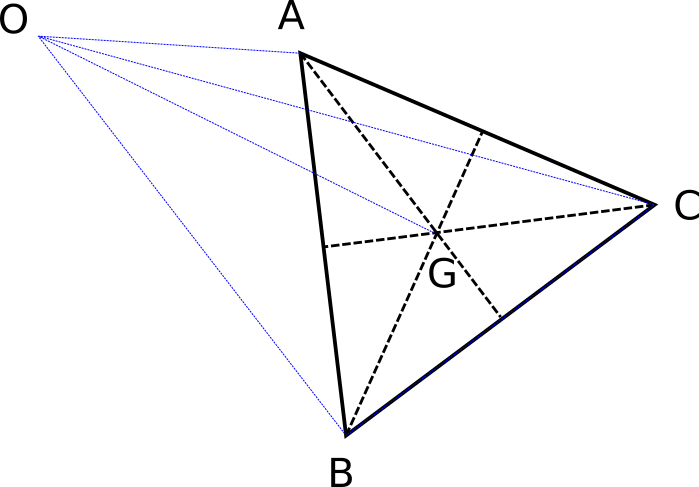
\includegraphics[scale=0.4]{tetra.png} 


\section{Notations}

\begin{itemize}
    \item $A$ is the point of observation
    \item $\eA$ is the associated vector
    \item $C$ is the local coordinate center of the 3d surface
    \item $D$ is the intersection of $(A, \eA)$ with the 3d surface
    \item $\eB$ is the associated reflected vector
    \item $\n(D)$ is the normal vector of the 3d surface at point $D$
\end{itemize}

\newpage
\section{General equations}


\subsection{intersection: finding $D$}

Point $D$ is such that:
$$
    \AD = k\eA = \AC + \CD
$$

So:
\begin{equation}
    k\eA\cdot\n = (\AC + \CD)\cdot \n
\end{equation}


\subsection{reflection: deriving angle of incidence}

The angle of incidence (with respect to the dioptre) is:
$$
    \alpha = \arcsin(-\eA \cdot \n)
$$

\subsection{reflection: deriving $\eB$}

The point $D$ on the 3d sufarce is such that $\n(D)$ is in the same plane as
$(A, D, B)$, which is written:

Using vector components:
$$
\begin{array}{lll}
    \eB
    & = (-\eA\cdot\n) \n + \left( \eA - (\eA \cdot \n)\n \right)\\
    & = \eA - 2(\eA\cdot\n) \n
\end{array}
$$

We can check that in both cases:

$$
\left\{
\begin{array}{lll}
    \eB \cdot (\eA \cross \n) = 0 & \text{  (coplanar)}\\
    \eB \cdot \n = -\eA \cdot \n & \text{  (same angle)}\\
\end{array}
\right.
$$


\newpage
\section{Plane}

If the 3d surface is a plane, then $\n$ is constant and does not depend on $k$.

The equations become:

$$
\begin{array}{llll}
    (1)
    & \Leftrightarrow &
    k\eA\cdot\n
    & = \AC\cdot\n\\
    & \Leftrightarrow &
    k = \frac{\AC\cdot\n}{\eA\cdot\n}
\end{array}
$$


\newpage
\section{Cylinder}

Consider a cylinder of axes $(O, \z)$, with $\z$  unit vector and radius $r$.
The equations become:

$$
\begin{array}{llll}
    (1)
    & \Leftrightarrow &
    k\eA\cdot\n
    & = \AO\cdot\n + \OD\cdot \n\\
    & \Leftrightarrow &
    k\eA\cdot\n
    & = \AO\cdot\n + \ud{OE}\cdot \n + \ED \cdot \n\\
    & \Leftrightarrow &
    k\eA\cdot\n
    & = \AO\cdot\n + \ED \cdot \n\\
    & \Leftrightarrow &
    k\eA\cdot\n
    & = \AO\cdot\n + (-r\n) \cdot \n\\
    & \Leftrightarrow &
    k\eA\cdot\n
    & = \AO\cdot\n - r\\
\end{array}
$$

Now, for any point on line $(A, \eA)$, the unit vector $\n$ is:
$$
\n(D) = \frac{(\OD \cross  \z) \cross \z}{
    \|(\OD \cross  \z) \cross \z\|
}
    = \frac{(\OD \cross  \z) \cross \z}{\ODz}
$$

And:
$$
\begin{array}{lll}
    & \OD \cross \z & = \OA\cross\z + k\eA\cross\z\\
    \Rightarrow &
    (\OD \cross \z) \cross \z
    & = (\OA\cross\z) \cross \z + k(\eA\cross\z) \cross \z
\end{array}
$$

And:
$$
\ODz^2 = \OAz2 + k^2\eAz2 + 2k(\OA\cross\z)\cdot(\eA\cross\z)
$$

So
$$
\begin{array}{llll}
    (1)
    & \Leftrightarrow &
    k\eA\cdot\n
    & = \AO\cdot\n - r\\
    
    & \Leftrightarrow &
    k\eA \cdot ((\OD \cross  \z) \cross \z)
    & = \AO \cdot ((\OD \cross  \z) \cross \z) - r\ODz\\
    
    & \Leftrightarrow &
    - k (\OD \cross  \z) \cdot (\eA \cross \z)
    & = (\OD \cross  \z) \cdot (\OA \cross \z) - r\ODz\\
    
    & \Leftrightarrow &
    r\ODz
    & = k (\OD \cross  \z) \cdot (\eA \cross \z)
    + (\OD \cross  \z) \cdot (\OA \cross \z)\\
    
    & \Leftrightarrow &
    r\ODz
    & = (\OD \cross  \z) \cdot (k\eA \cross \z + \OA \cross \z)\\
    
    & \Leftrightarrow &
    r\ODz
    & = \ODz^2\\
\end{array}
$$

But $\ODz \neq 0$ because $D$ cannot be of the axis of the cylinder.

So
$$
\begin{array}{llll}
    (1)
    & \Rightarrow &
    r^2 = \ODz^2\\

    & \Leftrightarrow &
    r^2 = \OAz2 + k^2\eAz2 + 2k(\OA\cross\z)\cdot(\eA\cross\z)\\
\end{array}
$$

So ultimately:
$$
\begin{array}{llll}
    (1)
    & \Rightarrow &
    k^2\eAz2 + 2k(\OA\cross\z)\cdot(\eA\cross\z) + \OAz2 - r^2 = 0\\
\end{array}
$$



\newpage
\section{Sphere}

Consider a sphere of center $O$ and radius $r$.
The normal vector associated to any point $E$ (not on $O$) is:

$$
\n(D) = - \frac{\OD}{\ODn}
$$

Given that $E$ in on the $(A, B)$ line:

Which is the same equation as for the cylinder, but with cross products
replaced by norms.
$$
\begin{array}{llll}
    (1)
    
    & \Leftrightarrow &
    k\eA\cdot\n
    & = \AO\cdot\n + \OD\cdot \n\\
    
    & \Leftrightarrow &
    k\eA\cdot\n
    & = \AO\cdot\n - r\\
    
    & \Leftrightarrow &
    -k\eA\cdot\OD
    & = -\AO\cdot\OD - r\ODn\\
    
    & \Leftrightarrow &
    r\ODn
    & = \OA\cdot\OD + k\eA\cdot\OD\\
    
    & \Leftrightarrow &
    r\ODn
    & = \ODn^2\\

    & \Rightarrow &
    r^2
    & = \ODn^2\\

    & \Leftrightarrow &
    r^2
    & = \|\OA\|^2 + k^2 + 2k\OA\cdot\eA\\
\end{array}
$$

So ultimately:
$$
\begin{array}{llll}
    (1)
    & \Rightarrow &
    k^2 + 2k\OA\cdot\eA + \|\OA\|^2 - r^2 = 0\\
\end{array}
$$


\newpage
\section{Torus}

Consider a torus of axes $(O, \z)$, with $\z$  unit vector.
It has major radius $\ra$ and minor radius $\rb$.

For any point $E$ in space, we have:

$$
    \ea(E) = - \frac{(\ud{OE} \cross  \z) \cross \z}{
    \|(\ud{OE} \cross  \z) \cross \z\|
}
$$



\end{document}
